\documentclass{article}
\usepackage{multicol}
\usepackage{graphicx}
\usepackage[toc,page]{appendix}
\usepackage[margin={3cm,3cm}]{geometry}
\usepackage[super,square]{natbib}
\usepackage{hyperref}
\usepackage{xcolor}
\hypersetup{
    colorlinks,
    linkcolor={red!50!black},
    citecolor={blue!50!black},
    urlcolor={blue!80!black}
}


\title{
FreezeNet \\
Making Proof-of-Work More Useful
}

\author{Téo Bouvard}

\date{}

\begin{document}

\maketitle

\begin{abstract}
	We propose an alternative to Hashcash challenges in proof-of-work protocols, with the goal of maximizing the computational usefulness of such protocols using neural network training.
\end{abstract}

\begin{multicols}{2}

	\section{Introduction}
	Proof-of-work is a consensus mechanism intended to deter denial-of-service attacks. The idea was first presented by Dwork and Naor\cite{Dwork93} in 1993, and was later formalized by Jackobsson and Juels\cite{Jakobsson99} in 1999.

	The concept behind proof-of-work is to propose a challenge which can be solved with a measurable difficulty, and which solution is easy to verify.

	An example implementation of a proof-of-work protocol is the Hashcash algorithm\cite{back02hashcash}, where the challenge is to find an integer value which, when appended to some given data, produces a hash digest inferior to a given target value. Because of the properties of cryptographic hash functions, the most efficient way to find a solution is to try random values until the resulting hash satisfies the given constraint. The difficulty of this challenge grows exponentially as the target value decreases. However, verifying a solution is fast and is constant-time with the challenge difficulty, as the only thing to do is to verify is that the hash of the concatenation of the data and the solution value yields a digest inferior to the target value.

	Derivatives of the Hashcash algorithm are used as consensus mechanisms for more than 470 cryptocurrencies \cite{cryptoslate20}. Despite its robustness, proof-of-work is virtually useless. The computational power needed to generate a solution to each challenge is never used again once the solution has been found. Moreover, this computational power is significant. According to the International Energy Agency\cite{ieabtcenergy20}, Bitcoin mining alone is estimated to use between 20 and 80 TWh of electricity annually, which represent the annual domestic electricity consumption of whole countries such as Portugal\cite{enerdata}.

	To make proof-of-work more useful, we try to replace Hashcash-like challenges with neural network training, which is also a computationally intensive task. Such a task would fulfill the requirements of a proof-of-work protocol : it is a computational challenge with a measurable difficulty having solutions which are easy to verify. Solutions to this kind of challenges could be verified using common metrics such as accuracy or F1-score on test datasets.

	However, this opens up a larger attack surface than Hashcash challenges. The main attack we try to prevent in this paper are transfer learning attacks. In this type of attack, a malicious party could pass verification tests, using a pre-trained model which was fine-tuned for the given task. To prevent such attacks, we need to devise a protocol where an attacker would have no incentive in using a pre-trained network, because it would not give him any advantage in solving the challenge.

	We present an approach using neural network training as an alternative to Hashcash-like challenges in proof-of-work protocols. This approach deter transfer learning attacks by embedding information in the network. This information is used as proof that the network was trained from scratch for a specific task, and can be verified along with the task metrics when a solution is submitted.

	\section{Experimental setup}

	We use the CIFAR-10 dataset, an image classification dataset containing 60,000 images belonging to 10 classes with a balanced distribution. The images are 32 $ \times $ 32 pixels with 3 color channels. We use 50,000 images for training, and 10,000 images for testing.


	\section{Watermarking procedure}

	In this approach, the main assumption is that we have read and write access to the weights inside the model. We use this assumption to derive a watermarking procedure which imposes strict constraints on some weights of the model. This procedure is used to verify that a neural network was trained with a specific watermark. The watermark is derived from some data, using a cryptographic hash function and a Pseudo Random Number Generator. The watermark can be thought of as a unique link tying a piece of data and a neural network together.

	\subsection{Creating a watermark}

	A watermark is created by hashing the data we want to embed in the solution, and using the resulting digest as a seed for a Pseudo Random Number Generator. We then use this PRNG to generate a sequence of weights of a fixed size. This sequence of weights is the watermark, and it uniquely identifies the embedded data.
	As an example, we could use the bytes representation of a blockchain block as the embedding data.

	\subsection{Applying a watermark}

	Having generated the watermark, we now need an encoding function to apply it to a neural network. Ideally, the encoding function should be structure agnostic, so that we could apply a watermark to a network without any constraints on its architecture.
	The encoding function we use is to randomly assign the watermark's weights to the model's weights. The placement of the watermark weights is determined by indices drawn from the same PRNG we previously used to generate the weights. This ties both the weights and their indices in the network to the embedded data, thus acting as a watermark. The watermark indices can be thought of as the indices of the model weights if they were sequentially flattened into a single one dimensional array.
	To apply the watermark, we simply replace the model weights at the watermark indices by the watermark weights.

	\subsection{Verifying a watermark}

	The verification process is similar to the watermarking process, except that we do not replace the weights but compute the difference between the watermark weights and the model weights. If this difference is below a given tolerance threshold, then the model is said to conform to the watermark. The tolerance is only introduced as an implementation side-effect, because of the intrinsic imprecision of floating point arithmetic. Theoretically, it would be sufficient to check for a strict equality between the watermark weights and the model weights.

	\subsection{Training with a watermark}

	In order to use this watermarking procedure in a proof-of-work protocol, we simply apply the watermark to the network at the end of each training batch. Each time the backpropagation algorithm has updated the weights, we apply the watermark. This incidentally forces the network to learn with a strict constraint on certain weights.

	\subsection{Results}

	To conduct the following experiments, we use a simple custom baseline model comprising of 4 convolution blocks and 2 fully connected layers. The general structure of this model is presented in \autoref{fig:modelstructure}.

	Each convolution block consists of 2 successive convolutions followed by a max-pool and a dropout. The number of filters and the dropout ratio are functions of the convolution block index, as shown in \autoref{fig:convblock}. This model achieves a test accuracy of 88.2\% after 100 training epochs. More implementation details can be found in the notebook and the code.

	The first result is that the network can still learn even when a significant proportion of its weights are constrained by the watermark. In \autoref{fig:watermark_training}, experimentation show that even when the watermark size is 70\% the number of weights in the model, the model reaches 65\% accuracy after 100 epochs. Moreover, it seems that the learning curve is not yet reaching a plateau. This is a desired behaviour as it shows that the difficulty of training the network is correlated with the size of the watermark. Thus, the proof-of-work difficulty can be tuned by setting the desired watermark size.

	\begin{figure*}[htbp]
		\centering
		\includegraphics[width=\textwidth]{assets/learning_ability_f1.png}
		\caption{Training from scratch with a watermark}
		\label{fig:watermark_training}
	\end{figure*}

	The second result is weak tampering resistance, where applying a watermark on a trained network decreases its predictive power according to an exponential decay with the watermark size. This shows that a plain model-reuse attack is not feasible if we set a watermark size large enough. In \autoref{fig:watermark_hit}, we observe that once the watermark size represents more than 10\% of the model weights, the baseline model accuracy drops to a random classification score.

	\begin{figure*}[htbp]
		\centering
		\includegraphics[width=\textwidth]{assets/weak_tampering.png}
		\caption{Pretrained model accuracy after watermarking}
		\label{fig:watermark_hit}
	\end{figure*}

	The third result is strong tampering resistance, where re-training a pre-trained model with a watermark does not gives a significant advantage in solving the proof-of-work challenge. In \autoref{fig:transfer_attack}, experiments show that there is no incentive for an attacker to use transfer learning because honest training from scratch is at least as efficient. We observe that in the first two-thirds of training, a pre-trained model learns faster, but this advantage fades as the accuracy gets higher. Furthermore, this head-start advantage is further reduced by increasing the watermark size. For a watermark size of 70\% of the model weights, honest training is nearly indiscernible from transfer attack, and the accuracy still reaches more than 60\% after 100 epochs.

	\begin{figure*}[htbp]
		\centering
		\includegraphics[width=\textwidth]{assets/strong_tampering.png}
		\caption{Transfer learning attack}
		\label{fig:transfer_attack}
	\end{figure*}

	\subsection{Possible Improvements}

	One possible improvement to this approach could be to apply the watermarked weights during the backpropagation, not after it has been performed. This would require lower-level access to the weights during the backpropagation algorithm, but it may lead to a faster learning curve.
	In our implementation, the weights are drawn from a uniform distribution in $ [-1, 1] $, and the indices are drawn from a uniform distribution in all possible model indices without replacement. This means that, for example, the probability of watermarking a weight in a hidden layer is the same as watermarking a weight in the output layer. It may be interesting to experiment with different strategies and distributions for generating these weights and indices.
	Another improvement would be to replace the two modules for hashing and generating weights by a single Deterministic Random Bit Generator derived from a hash function. In our case, we used SHA-256 as hash function to compute the seed, and initialized a Mersenne Twister PRNG with this seed. The alternative would be to use a Hash-DRBG\cite{barker_kelsey_2015} to directly generate weights from the hash function output, without having to use a separate PRNG.

	\section{Limitations}

	Unlike Hashcash challenges, using neural network training as proof-of-work adds a considerable overhead to the entire process. In practice, it requires the transfer of a dataset from a source to all workers in the network. Without introducing a way to generate these datasets in a decentralized manner, this process is inherently incompatible with fully distributed blockchains.
	The overhead is also significant when workers present their solution, as they have to transfer all weights in the model leading to their solution. However we can greatly reduce the number of weights they have to transfer, as a proportion of these weights are constrained by the watermark and can be recomputed locally from the embedded data. This improvement might not be very significant because the main overhead comes from the dataset transfer.

\end{multicols}

\begin{appendices}

	\begin{figure}[h!]
		\centering
		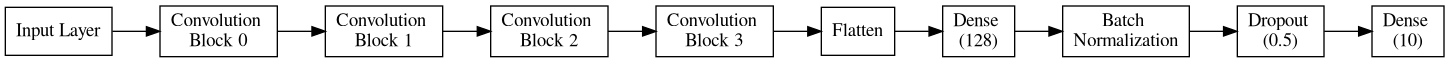
\includegraphics[width=\textwidth]{assets/model.png}
		\caption{General model structure}
		\label{fig:modelstructure}
	\end{figure}

	\begin{figure}[h!]
		\centering
		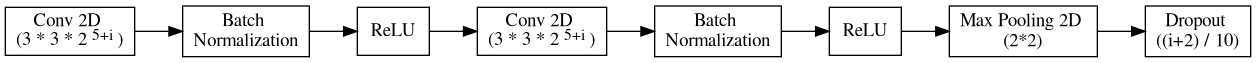
\includegraphics[width=\textwidth]{assets/convblock.png}
		\caption{Convolution block}
		\label{fig:convblock}
	\end{figure}

\end{appendices}

\bibliographystyle{unsrt}

\bibliography{references}

\end{document}